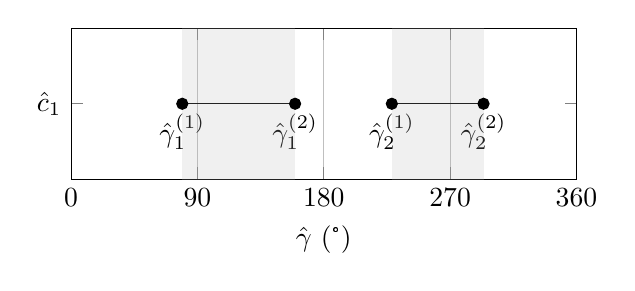
\begin{tikzpicture}
	\begin{axis}[height=3.5cm, width=8cm,xlabel={$\hat{\gamma}$ (\textdegree)}, xtick={0,90,180,270,360}, xmin=0, xmax=360, ytick={1}, yticklabels={$\hat{c}_1$},xmajorgrids]
	% Bogenspuren mit Kreis C_2
	\addplot[mark=*] plot coordinates  { (79.22,1) (159.59,1) } node[below, pos=0] {$\hat{\gamma}^{(1)}_{1}$} node[below, pos=1] {$\hat{\gamma}^{(2)}_{1}$};
	\draw[decoration={brace,raise=5pt,amplitude=3pt},decorate]
  (79.22,0) -- node[above=6pt] {$\hat{b}_{1}$} (159.59,0);
	\addplot[mark=*] plot coordinates { (228.49,1) (293.81,1) } node[below, pos=1] {$\hat{\gamma}^{(2)}_{2}$} node[below, pos=0] {$\hat{\gamma}^{(1)}_{2}$};
	\draw[decoration={brace,raise=5pt,amplitude=3pt},decorate]
  (228.49,0) -- node[above=6pt] {$\hat{b}_{2}$} (293.81,0);
	% Füge noch eine graue Box zur Kennzeichnung der übriggebliebenen Bogenstücken hinzu
	\fill [gray!60,fill opacity=0.2] (axis cs:79.22,0) rectangle (axis cs:159.59,2);
	\fill [gray!60,fill opacity=0.2] (axis cs:228.49,0) rectangle (axis cs:293.81,2);
	\end{axis}	
\end{tikzpicture}